\documentclass[final]{beamer}

\mode<presentation>
{
  \usetheme{CPC}
  \usefonttheme[onlymath]{serif}
}

% additional settings
\setbeamerfont{itemize}{size=\normalsize}
\setbeamerfont{itemize/enumerate body}{size=\normalsize}
\setbeamerfont{itemize/enumerate subbody}{size=\normalsize}

\usepackage{amsmath}
\usepackage[english]{babel}
\usepackage[utf8]{inputenc}
\usepackage[orientation=landscape,size=a0,scale=2]{beamerposter}

\usepackage{microtype}
\usepackage{color}
\usepackage{fancyvrb}

\usepackage{color}
\usepackage{listings}
\usepackage{bm}
\usepackage{calc}

\newcommand{\neghalfthinspace}{\kern -0.0833em}

\lstset{ %
  basicstyle=\ttfamily\small,  %
  breaklines=true, %
  keywordstyle=\textbf %
}

\DeclareMathOperator{\Var}{Var}
\DeclareMathOperator{\Covar}{Covar}


\title{User guided outlier detection in heterogeneous datasets}
\author{Clément Pit-\kern0pt-Claudel, Zelda Mariet, Rachael Harding}
\institute[MIT]{Massachusetts Institute of Technology}
\date{Dec. 10, 2014}

\newlength{\colwidth}
\newlength{\colswidth}
\newlength{\doublecolwidth}
\newlength{\blocksep}

\begin{document}
\begin{frame}[fragile]{}
  \setlength{\blocksep}{1.5ex}
  \setlength{\colwidth}{(\textwidth - 2\blocksep)/3}
  \setlength{\doublecolwidth}{2\colwidth + \blocksep}

  \begin{columns}[T,totalwidth=\textwidth]
    \begin{column}{\colwidth}
      \begin{block}{\thighlight{Motivation}}
  \begin{itemize}
  \item \highlight{Errors in data are extremely common}
    \begin{itemize}
    \item Human error, faulty sensors
    \end{itemize}
  \item \highlight{Errors can be hard to identify}
    \begin{itemize}
    \item Hidden data dependencies
    \item SQL datatypes have low expressivity
    \end{itemize}
  \item \highlight{Error tracking and elimination is expensive}
  \end{itemize}
\end{block}
 \vspace{\blocksep}
      \newcommand{\outlier}[1]{\textbf{#1}}
\begin{block}{\thighlight{Example: Outliers in the CSAIL directory}}
  \small
  \renewcommand{\arraystretch}{1.2}
  \setlength\tabcolsep{3\tabcolsep}
  \begin{tabular*}{\textwidth}{ l | l | l | l }
    Last name & First name & Office & Email \\
    \hline
    Harding & Rachael & \outlier{32-888} & rhardin@mit.edu \\
    Mariet & Zelda & 32-G414 & zmariet@mit.edu \\
    \outlier{Pit-claudel} & Clément & 32-G804 & cpitcla@mit.edu \\
  \end{tabular*}
\end{block}
 \vspace{\blocksep}
      \begin{block}{\thighlight{Our Approach}}
  \subttl{Tuple expansion}
  
  \texttt{\parbox{\widthof{1418222130}}{"32-G414"}} $\longrightarrow
  \begin{cases}
    \text{length: } & \texttt{7}\\
    \text{signature: } & \texttt{NNPLNNN}\\
    \text{uppercase: } & \texttt{True (1)}\\
  \end{cases}$
  
  \texttt{1418222130} $\longrightarrow
  \begin{cases}
    \text{date: } & \texttt{(2014,12,10)}\\
    \text{weekday: } & \texttt{Wed (2)}\\
    \text{binary: } & \texttt{0b10101\ldots010}\\
  \end{cases}$
  
  \subttl{3 pass pipeline}
  \begin{itemize}
  \item Statistical analysis
  \item Data modeling
  \item Outlier detection
  \end{itemize}
\end{block}
    \end{column}
    
    \begin{column}{\doublecolwidth}
      \begin{block}{\thighlight{Our pipeline}}
        \begin{figure}
          \centering
          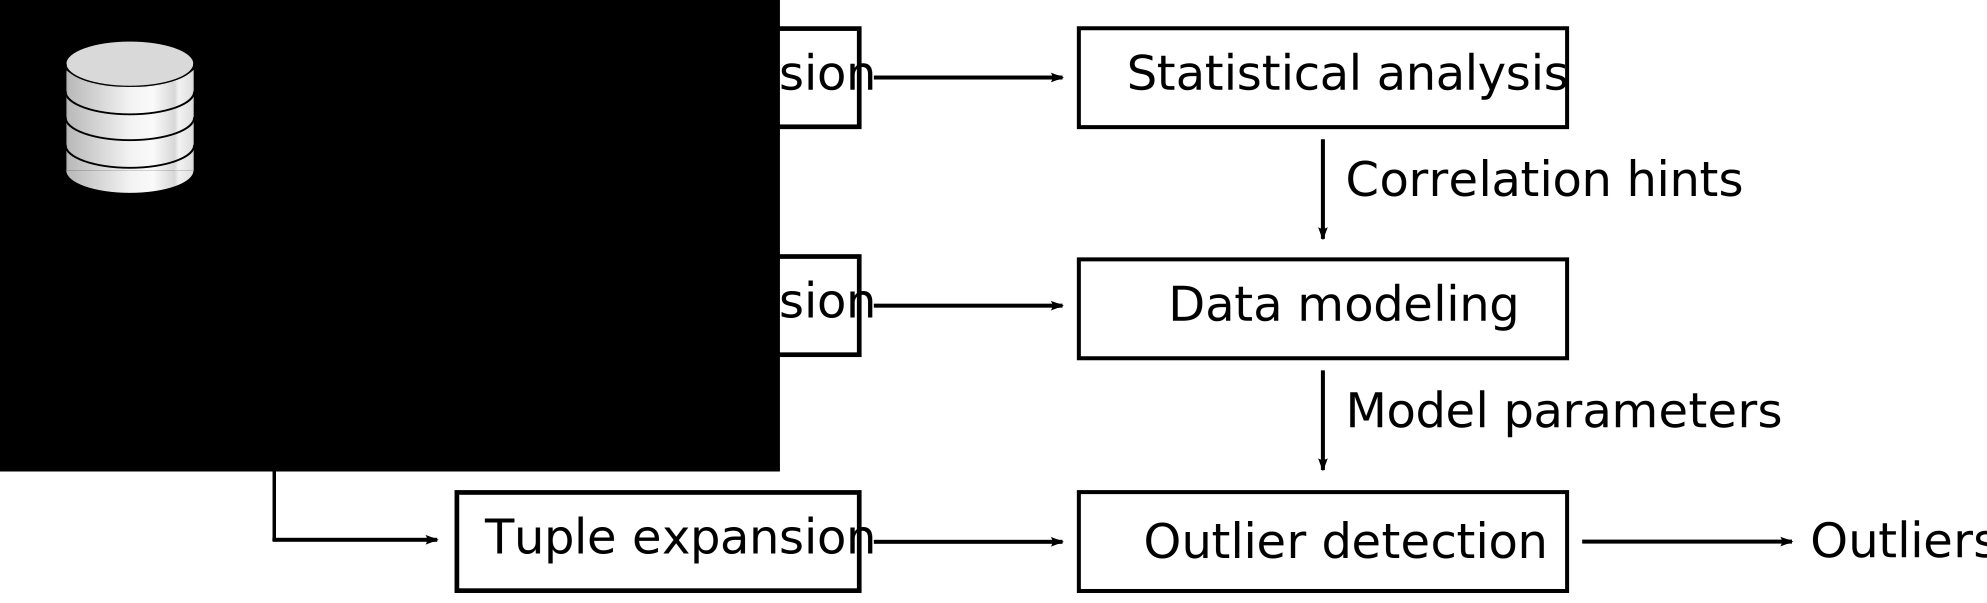
\includegraphics[width=\linewidth]{../graphics/pipeline.pdf}
        \end{figure}
      \end{block} \vspace{\blocksep}

      \vspace{-\baselineskip}
      \begin{columns}[t,totalwidth=\textwidth]
        \begin{column}{\colwidth}
          \newcommand{\picturecolumn}[2][1]{
    \begin{column}{.32\textwidth}
      \begin{figure}
        \centering
        \includegraphics[height=.75\linewidth,page=#1]{#2}
      \end{figure}
    \end{column}
}
\newcommand{\hsepline}{
  \par\vspace{-.75\baselineskip}
  \rule{0.9\linewidth}{1pt}
}

\begin{block}{\thighlight{Outliers characterization and detection}}
  \subttl{Statistical analysis}
  \begin{center}
    \begin{minipage}{.5\textwidth}
      \centering
      Pearson's correlation
      \hsepline{}
      Soft dependencies between numerical series
    \end{minipage}
  \end{center}
  
  \vspace{0.5\baselineskip}\subttl{Data modeling}
  \begin{columns}[T]
    \begin{column}{.32\textwidth}
      \centering
      Gaussian Model
      \hsepline{}
      Simple numerical data
    \end{column}
    
    \begin{column}{.32\textwidth}
      \centering
      Mixture Model
      \hsepline{}
      Multivariate numerical data
    \end{column}

    \begin{column}{.32\textwidth}
      \centering
      Histogram
      \hsepline{}
      Multivariate heterogeneous data
    \end{column}
  \end{columns}
  ~
  
  \subttl{Outlier Analysis}	
  \begin{columns}[T]
    \picturecolumn[1]{../graphics/models-plots-crop.pdf}
    \picturecolumn[2]{../graphics/models-plots-crop.pdf}
    \picturecolumn[3]{../graphics/models-plots-crop.pdf}
  \end{columns}
\end{block}
 \vspace{\blocksep}
        \end{column}

        \begin{column}{\colwidth}
          
\begin{block}{\thighlight{Evaluation: Intel Sensor Data}}
\vspace{-1cm}
\begin{itemize}
\item Sensors measure temp, humidity, light, and voltage
\item Sensor failure when voltage drops
\end{itemize}
        \begin{figure}
          \centering
          \includegraphics[width=\textwidth]{../graphics/sensors-crop.pdf}
          \caption{Gaussian Model and Mixture Model (Voltage vs. Temperature). Red points are detected outliers.}
        \end{figure}

\vspace{-1.5cm}
\end{block}
 \vspace{\blocksep}
          % \section{Future Work}
% \label{sec:future-work}
 \vspace{\blocksep}
        \end{column}      
      \end{columns}
    \end{column}      
  \end{columns}
\end{frame}
\end{document}